\section{Subsystem Decomposition}
We have defined the following subsystems:
\begin{itemize}
	\item \textbf{Persistence subsystem (EntityFramework):} This sub system manages storing and retrieving Entity objects using the Entity Framework and its serialisation functionality.\\
	The serialised Entities are stored in a Microsoft SQL database which is hosted on Microsoft Azure. The sub system provides the \texttt{DriveIT Web API} (mentioned below) deserialised Entities, which uses these to provide the backend for other sub systems using the API.\\
	The subsystem supports retrieving all Entities of a given type, a specific Entity using its unique ID and retrieving an Entity on its relation to other Entities. 
	\begin{figure}[H]
		\centering
		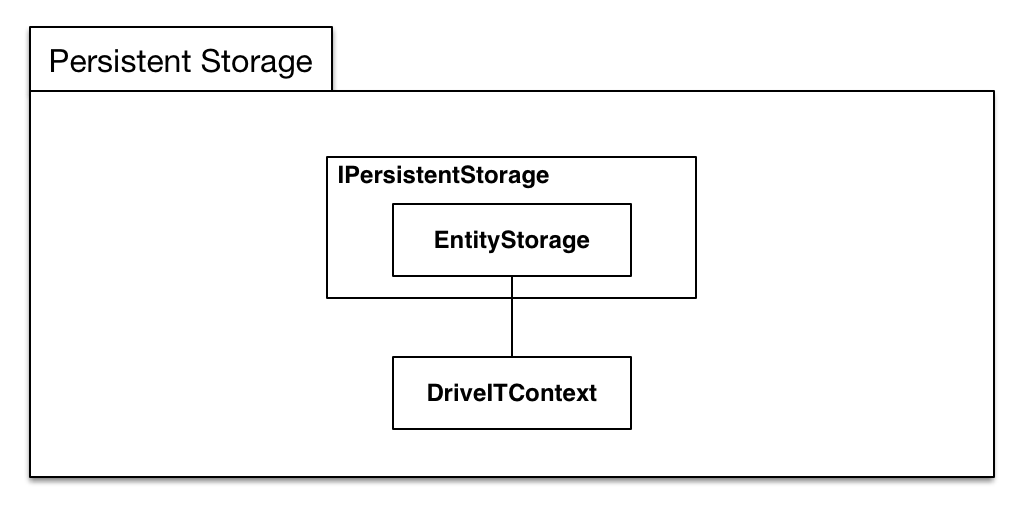
\includegraphics[scale=0.30]{Figures/EntityFrameworkSubsystemDecomposition}
		% place the figure in the Figures folder (located with the main file)
		% you need to fix the scale a few times to get it right, but latex does not compress so one can always zoom in to see details.
		\caption{Subsystems of the EntityFramework Subsystem.}
	\end{figure}
	\item \textbf{WebAPI:} The \texttt{DriveIT Web API} provides public communication with the persistence subsystem and also handles authorisation of users of the sub system.\\
	The subsystem provides access to the persistence sub system using specific URL routes and enforces authorisation so unauthorized users only have limited access to the data of the \texttt{DriveIT System}.\\ 
	Every table in the persistence module must therefore be supported by the sub system, though not every table is available to every user.\\
	The \texttt{DriveIT Web API} is comprised of a series of modules for serialising the Model Entities into \texttt{JavaScript Object Notation (JSON)} and transferring these via a texttt{REST} interface accessible using \texttt{HTTP}. \\
	These modules are implemented using the \texttt{ASP.NET} framework, since these provide a lot of the neccessary funtionality out of the box, and simplify and shortens development time.
	\item \textbf{WindowsApp:} Used by the employees to serve the customers. The Windows application can only be accessed by employees who will have to login at startup. The application is used to CRUD cars, orders, customers and employees (by the administrator account-type).
	\item \textbf{CarQuery:} This subsystem is a collection of classes that enable the rest of the \texttt{DriveIT System} to fill out missing information about cars from the CarQuery API.\\
	The sub system is used by an employee when creating a new car. The subsystem mainly consists of a \texttt{JSON} deserialiser that communicates with the \texttt{CarQuery REST API} and another class that receives a Car object and fills out the missing attributes using the deserialised JSON data. \\
	The employee fills out the information he/she knows about the car and the system then narrows its information search against the \texttt{CarQuery REST API}.
	\begin{figure}[H]
		\centering
		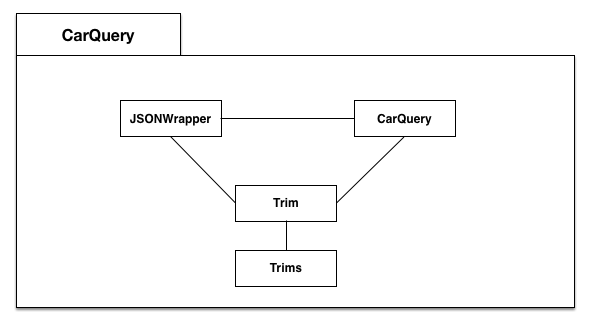
\includegraphics[scale=0.30]{Figures/CarQuerySubsystemDecomposition}\\
		% place the figure in the Figures folder (located with the main file)
		% you need to fix the scale a few times to get it right, but latex does not compress so one can always zoom in to see details.
		\caption{Subsystems of the CarQuery Subsystem.}
	\end{figure}
\end{itemize}